
\documentclass[12pt]{scrartcl}
\title{COL341 : HOMEWORK-2}
\nonstopmode

\usepackage{graphicx} % Required for including pictures
\usepackage[figurename=Figure]{caption}

\usepackage{float}    % For tables and other floats
\usepackage{verbatim} % For comments and other
\usepackage{amsmath}  % For math
\usepackage{amssymb}  % For more math
\usepackage{fullpage} % Set margins and place page numbers at bottom center
\usepackage{paralist} % paragraph spacing
\usepackage{listings} % For source code
\usepackage{subfig}   % For subfigures
%\usepackage{physics}  % for simplified dv, and 
\usepackage{enumitem} % useful for itemization
\usepackage{siunitx}  % standardization of si units

\usepackage{tikz,bm} % Useful for drawing plots
%\usepackage{tikz-3dplot}

\usepackage{setspace}
\usepackage{geometry}

\usepackage{amssymb} % for logic symbols
\usepackage{proof}
\usepackage{bussproofs}

\usepackage{natded}
\usepackage{prftree}

 \geometry{
 left=20mm,
 top=10mm,
 bottom=10mm,
 }

\Large


\begin{document}
\begin{center}
	\hrule
	\vspace{.4cm}
	{\textbf { \large COL703 Logic For CS SEM I 2023-24}}
\end{center}
\textbf{Name:}\ Vatsal Jingar {\hspace{\fill} \textbf{Date:} September 2023
}
{ \hspace{\fill} \textbf{Assignment-1} \\
	\hrule
}
% \onehalfspacing
\section{Question 1}
\subsection{Insertion Rule :}

$$
\prftree[r]{\text{$\leftrightarrow\mathrm{I}$}}
{\prfsummary{\phi}{\psi},}
{\prfsummary{\psi}{\phi}}
{\phi \leftrightarrow \psi}
$$

\subsection{Elimination Rules}:
\subsubsection{Elimination 1 } :

\begin{displaymath}
\prftree[r]{\text{$\leftrightarrow\mathrm{E}_{1}$}}
{\phi,}
{\phi \leftrightarrow \psi}
{\psi}
\end{displaymath}

\subsubsection{Elimination 2 } :

\begin{displaymath}
\prftree[r]{\text{$\leftrightarrow\mathrm{E}_{2}$}}
{\psi,}
{\phi \leftrightarrow \psi}
{\phi}
\end{displaymath}

\newpage
\subsection{Insertion Rule Derivation :}
\[
\Jproof{
    \cablk{
    \cablk{
        \proofline{\phi}{Assumption}
        \proofline{.}{R1}
        \proofline{\psi}{R2}
    }    
    \cablk{
        \proofline{\psi}{Assumption}
        \proofline{.}{R3}
        \proofline{\phi}{R4}
    }
    \proofline{\phi \rightarrow \psi}{\text{$\rightarrow_{I}(1-3)$}}
    \proofline{\psi \rightarrow \phi}{\text{$\rightarrow_{I}(4-6)$}}
    \proofline{(\phi \rightarrow \psi)\wedge(\psi \rightarrow \phi)}{\text{$\wedge_{I}(7\text{,}8)$}}
    }
}
\]
\subsection{Elimination Rule Derivation 1 : }
\[
\Jproof{
    \cablk{
    \proofline{(\phi \rightarrow \psi)\wedge(\phi \rightarrow \psi)}{Premise}
    \proofline{\phi}{Premise}
    \proofline{\phi \rightarrow \psi}{\text{$\wedge_{E1}(1)$}}
    \proofline{\psi}{\text{MP(2,3)}}
    }
}
\]
\subsection{Elimination Rule Derivation 2 : }
\[
\Jproof{
    \cablk{
    \proofline{(\phi \rightarrow \psi)\wedge(\phi \rightarrow \psi)}{Premise}
    \proofline{\psi}{Premise}
    \proofline{\psi \rightarrow \phi}{\text{$\wedge_{E2}(1)$}}
    \proofline{\phi}{\text{MP(2,3)}}
    }
}
\]

\newpage
\section{Question 2}
\subsection{Part a}
$(p \rightarrow r)\wedge(q \rightarrow r) \vdash p \wedge q \rightarrow r$
\[
\Jproof{
    \cablk{
    \proofline{(p \rightarrow r)\wedge(q \rightarrow r)}{Premise}
    \proofline{p \rightarrow r}{\text{$\wedge_{E1}(1)$}}
    \proofline{q \rightarrow r}{\text{$\wedge_{E2}(1)$}}
    \cablk{
    \proofline{p \wedge q}{Assumption}
    \proofline{p}{\text{$\wedge_{E1}(4)$}}
    \proofline{p \rightarrow r}{copy 2}
    \proofline{r}{MP 5,6}
    }   
    \proofline{p \wedge q \rightarrow r}{\text{$\rightarrow_{I}(4-7)$}}
    }
}
\]

\subsection{Part b}
$p \rightarrow q \wedge r \vdash (p \rightarrow q)\wedge(p \rightarrow r)$
\[
\Jproof{
    \cablk{
    \proofline{p \rightarrow q \wedge r}{Premise}
    \cablk{
        \proofline{p}{Assumption}
        \proofline{q \wedge r}{M.P 2,1}
        \proofline{q}{\text{$\wedge_{E1}(3)$}}
    }
    \proofline{p \rightarrow q}{\text{$\rightarrow_{I}(2-4)$}}
    \cablk{
        \proofline{p}{Assumption}
        \proofline{q \wedge r}{M.P 6,1}
        \proofline{r}{\text{$\wedge_{E2}(7)$}}
    }
    \proofline{p \rightarrow r}{\text{$\rightarrow_{I}(6-8)$}}
    \proofline{(p \rightarrow r)\wedge(q \rightarrow r}{\text{$\wedge_{I}(5,9)$}}
    }
}
\]


\newpage
\section{Question 3}
Let $\Phi$ be the set of well-formed formulas created by the set of atoms and $\{\leftrightarrow,\lnot\}$.
\begin{itemize}
    \item L($\phi$) = Number of literals present in the formula. It could be also defined as creating a parse tree and counting number of leaves (It would only give count of literals. Not necessary that leaves would be literals). Here $\phi \epsilon \Phi$
    \item Formulas with L($\phi$) = 1
    \begin{enumerate}
        \item Observation 1 : Possible cases are either they are negation of atom or atom itself. In both cases we will observe that number of True values are odd.
        \item Observation 2 : Another observation we will make is that for any truthtable, we will have $2^{n}$, $n \geq 0$ possible valuations. So total possible valuations are always even. Hence number of True values and number of False values are both even or both odd.
        \item Observation 3 : formula made by only connective as $\neg$ $\leftrightarrow$ literal (defined according to Huth and Ryan). This is because negation is unary operator. And for the other side as the second connective in set is binary we will always need two literals atleast.
        \item  Unary Operator $\neg$ applied on formula, if number of True values are even, then $\neg (\phi)$ will also have even True values. This is because by observation 2, False values in original formula would also be even. By negating all false values, they will become True in new formula. As false values are even, True values would also be even.
    \end{enumerate}
    \item Claim : For a formula $\phi$ with $L(\phi) > 1$, number of True values will be even if $\phi \epsilon \Phi$.
    \begin{enumerate}
        \item We will prove the claim using Induction over length of formula by the notion of length defined above.
        \item Base case : $L(\phi)=2$ ; For this case we can consider the possible structures of formula itself. 
        \item \begin{cases}
            p $\leftrightarrow$ p : Computing True values for it, we have 2 Trues.\\
            p $\leftrightarrow$ q : Here q is independent of p. Total True values are 2.\\
            p $\leftrightarrow$ $\neg p$ : Total True values are 0.\\
        \end{cases}
        \item Induction Hypothesis : For any formula of length $L(\phi) \leq k$, where $k > 2$, we assume that it contains even number of True values.
        \item Induction Statement : 
        \item \begin{itemize}
            \item We will calculate True values for any formula $\phi$ with $L(\phi)=k+1$.
            \item The structure of $\phi$ could be either $\neg \phi_{1}$ or $\phi_{1} \leftrightarrow \phi_{2}$
            \item Case 1 : $\phi = \neg \phi_{1}$
            \item By Observation 4, we can say that number of True values will be yet Even.
            \item Case 2 : $\phi = \phi_{1} \leftrightarrow \phi_{2}$
            \item Case 2.1 : This is possible that atmost one of them either $\phi_{1}$ or $\phi_{2}$ is of length 1. Consider $\phi_{1}$ of Length 1 WLOG.
            \item Consider the Truth table for this. Let the number of possible valuations in $\phi_{1}$ be n.
            \item By observation 3, we know that $\phi_{2}$ is literal. This means it contains 1 True value and 1 False value.
            \item To create the Truth table for $\phi$, Every True value of $\phi_{2}$ will occur $n \times m$, where m = number of True values in $\phi_{2}$.
            \item As n is even, Number of True values that would occur in Truth Table of $\phi_{2}$ will be even.
            \item Now its remains to show that if two formula with even true values are connected by $\leftrightarrow$ then they will have even number of true values.
            \item Assume the following :\\ Number of True values occurring in $\phi_{1}=a_{1}$\\ Number of False values occurring in $\phi_{1}=b_{1}$\\ Number of True values occurring in $\phi_{2}=a_{2}$\\ Number of True values occurring in $\phi_{2}=b_{2}$
            \item Now if both these are combined then consider the True False pairs created using the True values of $\phi_{1}$ be x. And number of True False pairs created using True values of $\phi_{2}$ be y.
            \item So number of True values remained for pairing with True values are : In $\phi_{1}$ It would be $a_{1}-x$ and In $\phi_{2}$ It would be $a_{2}-y$.
            \item They will be equal giving that x$-$y = even.
            \item Total number of valuations with True True pairs and False False pairs is Total valuations $-$ $(x+y)$.
            \item As Total valuations is always even, If $(x+y)$ would be even, we are done.
            \item As we know that $x-y$ is even, this means that x and y both are even or both are odd.
            \item In both possible cases, $(x+y)$ is even.
            \item Hence Proved the Claim
        \end{itemize}
        \item By this claim, We can state that as we are not able to create boolean funcitons of all the type, the set is not adequate. This is because this property is not satisfied by adequate set.
    \end{enumerate}
    
\end{itemize}




\newpage
\section{Question 4}
\subsection{Part a}
$\neg r \rightarrow (p \vee q),r \wedge (\neg q) \vdash r \rightarrow q$
\begin{figure}[H]
    \centering
    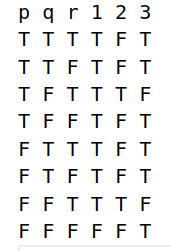
\includegraphics[scale=0.6]{Part1.png}
    \caption{Truth Table}
    \label{fig:enter-label}
\end{figure}
\begin{itemize}
    \item 1 in Table : $\neg r \rightarrow (p \wedge q)$
    \item 2 in Table : $r \wedge (\neg q)$
    \item 3 in Table : $r \rightarrow q$
\end{itemize}
\begin{itemize}
    \item It is visible from line no. 4, p = T, q = F, r = T is satisfying Formula 1 and 2 (giving truth values for them). While Formula 3 is not true for that.
\end{itemize}

\subsection{Part b}
$p \rightarrow (q \rightarrow r) \vdash p \rightarrow (r \rightarrow q)$
\begin{figure}[H]
    \centering
    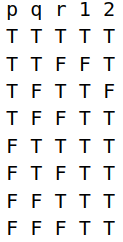
\includegraphics[scale=0.6]{Part2.png}
    \caption{Truth Table}
    \label{fig:enter-label}
\end{figure}

\begin{itemize}
    \item 1 in Table : $p \rightarrow (q \rightarrow r)$
    \item 2 in Table : $p \rightarrow (r \rightarrow q)$
    \item It is visible from line no. 4, that p = T, q = F, r = T. And for this Formula 1 is satisfying (giving true value). But for Formula 2, we are getting false.
\end{itemize}


\section{Question 5}
\subsection{Part a}
Set of all formulas $\Phi = \{\alpha_{0},\alpha_{1},..\}$\\
Given : X is a FSS\\
\textbf{Construction : }\\
\begin{itemize}
    \item $X_0$ = $X$
    \item $X_{i+1}$ = \begin{cases}
        $X_i \cup \{\alpha_{i}\}$ if $X_i \cup {\alpha_{i}}$ is FSS\\
        $X_{i}$ else
    \end{cases}
    \item  Y = $\cup_{i \geq 0}X_{i}$
\end{itemize}
\begin{enumerate}
    \item Claim 1 : Y is FSS
    \begin{itemize}
        \item We will prove this by contradiction.
        \item  Assume Y is not a FSS.
        \item By the definition of FSS, if Y is not a FSS, $\exists$ a Z $\subseteq_{fin}$ Y, which is not satisfiable.
        \item Let Z = ${\alpha_{i_{0}},\alpha_{i_{1}}....,\alpha_{i_{k}}}$
        \item  Here $i_{0} \leq i_{1} ...\leq i_{k}$
        \item As $Z \subseteq Y$, and $\alpha_{i_{k}} \epsilon Z$, we can say that $X_{i_{k}+1} = X_{i_{k}} \cup \{\alpha_{i_{k}}\}$. Because $\alpha_{i_{k}}$ could be present in Y only if it is added $i_{k}+1$ step.
        \item As $Z \subseteq Y$, and max index formula present in Z is $\alpha_{i{k}}$, we can say that $Z \subseteq X_{i_{k}+1}$. This is because $i_{0} \leq i_{1} .. \leq i_{k}$. If $\alpha_{i_{j}} \epsilon Z$, we know that $\alpha_{i_{j}}$ is added at $i_{j}+1$ step. Also, $X_{0} \subseteq X_{1} ... \subseteq X_{i_{k}+1}$
        \item We know that if $\alpha_{i_{k}}$ is added at $i_{k}+1$ step, then $X_{i_{k}} \cup \{\alpha_{i_{k}}\}$ is FSS. As it is FSS, every finite subset is satisfiable. Hence Z should be satisfiable.
        \item  This is Contradiction.
        \item Hence Y is FSS.
        
    \end{itemize}
    \item Claim 2 : Y is Maximal FSS
    \begin{itemize}
    \item  Suppose Y is not Maximal FSS.
    \item  Then $Y \cup \{\alpha_{i}\}$ for some $\alpha_{i} \epsilon \Phi/Y$, is FSS.
    \item  If $\alpha_{i}$ does not belong to Y, it must not be added at $i^{th}$ step. 
    \item  This meant that $X_{i} \cup \{\alpha_{i}\}$ was not FSS.
    \item  If $X_{i} \cup \{\alpha\}$ is not FSS, $\exists Z \subseteq_{fin} X_{i} \cup \{\alpha_{i}\}$ is not FSS.
    \item  As $Z \subseteq Y \cup \{\alpha_{i}\}$, and Z is not FSS. This contradicts that Y is FSS.
    \end{itemize}
    \item  Hence Y is maximal FSS.
\end{enumerate}

\subsection{Part b}
\begin{enumerate}
    \item Claim 1 : {$\alpha$,$\neg \alpha$} is not FSS.
    \begin{itemize}
        \item We know by LEM, $\alpha \vee \neg \alpha$ is valid. Hence $\neg(\alpha \vee \neg \alpha)$ is not satisfiable. As $\neg(\alpha \vee \neg \alpha)$ = $(\alpha \wedge \neg \alpha)$,
        \item  $(\alpha \wedge \neg \alpha)$ is not satisfiable.
    \end{itemize}
    \item Claim 2 : At least one of $\alpha$ or $\neg \alpha$ is in X.
    \begin{itemize}
        \item We will proof this by contradiction.
        \item Suppose neither of them belongs to X.
        \item As X is Maximal FSS, $\exists Y,Z \subseteq_{fin} X$, where $Y \cup \{\alpha\}$ and $Z \cup \{\neg \alpha\}$ is not satisfiable.
        \item Let Y = {$\beta_1$,$\beta_2$,...,$\beta_m$} and Z = {$\gamma_1$,...$\gamma_n$}.
        \item As $Z \cup \{\neg\alpha\}$ is not satisfiable $\implies$ $\gamma1 \wedge \gamma2... \wedge \neg \alpha$ is not satisfiable.
        \item Let $\beta = \beta_1 \wedge ... \beta_m$
        \item  Let $\gamma = \gamma_1 \wedge ... \gamma_n$
        \item  And similarly, $\beta1 \wedge \beta2... \wedge \alpha$ is not satisfiable.
        \item As we know that satisfiability is equivalent to consistency.
        \item $\vdash \neg(\alpha \wedge \beta)$ and $\vdash \neg(\neg \alpha \wedge \gamma)$
        \item As $\vdash \neg(\alpha \wedge \beta)$ = $\vdash \neg \alpha \vee \neg \beta$ = $\vdash \alpha \rightarrow \neg \beta$
        \item  Similarly, $\vdash \neg(\neg \alpha \wedge \gamma)$ = $\vdash \alpha \vee \neg \gamma$ = $\vdash \neg \alpha \rightarrow \neg \gamma$
        \item Sub-Claim : $\alpha \rightarrow \neg \beta, \neg \alpha \rightarrow \neg \gamma \vdash \neg \beta \rightarrow \gamma$
        \item Deduction Theorem,  $\alpha \rightarrow \neg \beta, \neg \alpha \rightarrow \neg \gamma, \neg \beta \vdash \gamma$
        \item M.T  $\alpha \rightarrow \neg \beta, \neg \alpha \rightarrow \neg \gamma, \neg \beta \vdash \neg \alpha$
        \item M.P $\alpha \rightarrow \neg \beta, \neg \alpha \rightarrow \neg \gamma, \neg \beta, \neg \alpha \vdash \neg \gamma$
        \item Hence Sub Claim Proved.
        \item As $(\neg \beta \rightarrow \neg \gamma) = (\neg \beta \vee \neg \gamma) = \neg(\beta \wedge \gamma)$
        \item As $(Y \cup Z)$ contains both $\alpha$ and $\neg \alpha$. And by Claim 1 proven above, it is not satisfiable,
        \item Hence $(Y \cup Z)$ is not FSS.
        \item This is contradiction.
        \item Hence, Atleast one of them is in X.
        
        
    \end{itemize}
    \item Both these properties, prove the claim that $\alpha \epsilon X \leftrightarrow \alpha \not \epsilon X$ 
\end{enumerate}
\subsection{Part c}
\begin{enumerate}
    \item "$=>$"
    \begin{itemize}
    \item Suppose $\alpha \vee \beta \epsilon X$, X is Maximal FSS.
    \item By the previous part (b), we know that atleast of the $\alpha$ or $\neg \alpha$ is in X.
    \item Suppose $\alpha$ is in X, then it proves the side.
    \item Suppose $\neg \alpha$ is in X.
    \item Given that $\alpha \vee \beta$ is in X, which is equivalent to $\neg \alpha \rightarrow \beta$.
    \item We will prove that if $\beta$ is not in X, then X is not a Maximal FSS.
    \item This could be done by proving that $X \cup \{\beta\}$ is FSS.
    \item Consider $Y = (X \cup \{\beta\})$
    \item We will prove Y as FSS
    \item Now Suppose Y is not a FSS
    \item Then by Satisfiability Lemma, $\exists Z \subseteq_{fin} Y$ which is not satisfiable
    \item It is easy to see that Z will contain $\beta$ otherwise $Z \subseteq_{fin} X$, As X is FSS, Z would be satisfiable. Hence Z must contain $\beta$.
    \item Let Z = $\{\beta,\gamma_{0},..,\gamma_{m}\}$
    \item We can also write that $\neg (\beta \wedge \gamma)$ is valid. As Z is not satisfiable.
    \item As $\neg \alpha$ and $\neg \alpha \rightarrow \beta$ are in X they are satisfiable.
    \item We know that $\{\gamma_{0},...,\gamma_{m},\neg \alpha,\neg \alpha \rightarrow \beta\}$ is satisfiable. As it is finite subset of X.
    \item We will show $\gamma_{0},...,\gamma_{m},\neg \alpha,\neg \alpha \rightarrow \beta \vdash \beta \wedge \gamma$
    \item Here $\gamma=\gamma_{0},\gamma_{1},..,\gamma_{m}$ 
    \item By showing this we can say that $\beta \wedge \gamma$ is satisfaible (As Hilbert System is complete So Satisfiability of Premises imples Satisfiablity of Provable Formulas), we can say that $\neg (\beta \wedge \gamma)$ is not valid, which will lead to contradiction.
    \item Proof of $\gamma_{0},...,\gamma_{m},\neg \alpha,\neg \alpha \rightarrow \beta \vdash \beta \wedge \gamma$ :
    \item M.P $\beta$
    \item (Premise) $\gamma$
    \item ($\wedge_{i}$) $\beta \wedge \gamma$
    \item As we know that all premises are satisfiable, there will exist some valuations for which $\beta \wedge \gamma$ will be satisfied, Hence it is satisfiable.
    \item So we reached to contradiction.
    \item Hence Y is FSS.
    \item Hence Proved.
    \end{itemize}
    \item $"<="$
    \begin{itemize}
        \item Given that $\alpha$ is in X
        \item We will prove that if $\alpha \vee \beta$ is not in X then X is not maximal FSS
        \item We will prove this by proving that $X \cup \{\alpha \vee \beta\}$ is FSS
        \item Let $Y = X \cup \{\alpha \vee \beta\}$
        \item Suppose Y is not FSS
        \item Then $\exists Z \subseteq_{fin} Y$ not satisfiable and Z must have $\alpha \vee \beta$ by the argument same as used in provinig the other side
        \item Now, Suppose $Z = \{\alpha \vee \beta, \gamma\}$, where $\gamma = \gamma_{0},\gamma_{1},..,\gamma_{m}$
        \item As Z is not satisfiable, we can say that $\neg((\alpha \vee \beta) \wedge \gamma)$ is valid
        \item Now as $\alpha$ and $\gamma$ is in X, $\{\alpha,\gamma\}$ is satisfaible as it is a finite subset of X.
        \item It is easy to see that $\alpha,\gamma \vdash (\alpha \vee \beta) \wedge \gamma$
        \item As "or" insertion and "and" insertion can be proven in Hilbert System.
        \item We know that as Left side (premises) are satisfaible
        \item As Hilbert System is complete. We have $\alpha,\gamma \models (\alpha \vee \beta) \wedge \gamma$
        \item This shows that $(\alpha \vee \beta) \wedge \gamma$ is satisfaible, Hence $\neg((\alpha \vee \beta) \wedge \gamma)$ is not valid.
        \item This is a contradiction.
        \item Hence Y is FSS
    \end{itemize}
    \item This proves the claim.
\end{enumerate}
\subsection{Part d}
\begin{enumerate}
    \item Let us assume that $v_{\alpha}$ is set of all possible valuations for which $\alpha$ has a valuation of True.
    \item Here $\alpha \epsilon X$
    \item For any $Z \subseteq X$, we will define $v_{Z} = \cap_{\alpha \epsilon Z}(v_{\alpha})$
    \item We will define $v^{*} = \cap_{\alpha \epsilon X}v_{\alpha}$
    \item This is observable that $v_{*}$ is non empty. Otherwise If it is empty, then $\exists Z \epsilon X$ which is empty (By Konnigs Lemma).
    \item And as X is FSS, Z must be satisfiable but if $v_{Z}$ is empty then there exist no valuation such that $v_{Z}$ could be True.
    \item This contradicts our Assumption, Hence $v^{*}$ is not empty.
    \item Now we will prove that $\exists v_{x} \epsilon v^{*}$ such that $v_{x} \models \alpha \leftrightarrow \alpha \epsilon X$
    \item $"<="$
    \begin{itemize}
        \item As $v^*$ is intersection over all possible valuations $\forall \alpha \epsilon X$, It must be a subset of $v_{\alpha} \forall \alpha$
        \item So $v_{x} \models \alpha$
        \item Hence Proved
    \end{itemize}
    \item $"=>"$
    \begin{itemize}
        \item Suppose $\alpha \not \epsilon X$
        \item By the part b, if $\alpha \not \epsilon X$ then $\neg \alpha \epsilon X$
        \item As $\neg \alpha \epsilon X$, By $"<="$ direction we can say that $v_{x} \models \neg \alpha$
        \item But we know that $v_{x} \models \alpha$, which is a contradiction.
        \item Hence $\alpha \epsilon X$
    \end{itemize}
    \item This proves the claim
\end{enumerate}

\subsection{Part e}
\begin{enumerate}
    \item By part d, we know that $\alpha \epsilon X \leftrightarrow v_{x} \models X$, if X is maximal FSS, $\forall \alpha$
    \item For any FSS, Y we can construct a maximal FSS $X_0$.
    \item So $Y \subseteq X$
    \item As $v_{x} \models \alpha$ $\forall \alpha \epsilon X_{0}$.
    \item So,$v_{x} \models \alpha$ $\forall \alpha \epsilon Y$, as $Y \subseteq X_{0}$.
    \item Let Y' = Any finite subset of Y
    \item So, $v_{x} \models \wedge_{\alpha \epsilon Y'}\alpha$
    \item As all the finite subsets of Y are satisfiable by only valuation $v_{x}$.
    \item Y is simultaneously satisfiable
\end{enumerate}

\subsection{Part f}
\begin{enumerate}
    \item ($<=$):
    \begin{itemize}
        \item If $Y \subseteq_{fin} X$, and $Y \models \alpha$.
        \item $Y \cup Z \models \alpha$, $\forall Z$
        \item Let $Z = X/Y$
        \item $X \models \alpha$
        \item As $v \models X$ then $v \models Y$.
        \item As $Y \models \alpha$.
        \item By logical sequence, $v \models \alpha$
    \end{itemize}
    \item ($=>$)
    \begin{itemize}
        \item Sub-Claim : For all $Z \subseteq \Phi$ and all $\beta \epsilon \Phi$, $Z \models \beta$ iff $Z \cup \{\neg \beta\}$ is not satisfiable.
        \item Sub-Claim Proof : If Z is not satisfiable, then we are done. If Z is satisfiable and $Z \cup \{\neg \beta\}$ is also satisfiable. As $Z \models \beta$, then $Z \cup Y \models \beta$ for $Z \cup Y$ begin satisfiable. As $Z \cup \{\neg \beta\}$ is satisfiable,  $Z \cup \{\neg \beta\} \models \beta$. This is contradiction. Hence sub claim proven.
        \item Suppose $X \models \alpha$.
        \item By sub claim $X \cup \{\neg \alpha\}$ is not satisfiable. As proven in class, if X is satisfiable then all its finite subset are satisfiable by konigs lemma. As $X \cup \{\neg \alpha\}$ is not satisfiable, $\exists Y \subseteq_{fin} X$ not satisfiable. As Y could be rewritten as $(Y/\{\neg \alpha\}) \cup \{\alpha\}$, which is not satisfiable, by sub claim, we can say that $(Y/\{\neg \alpha\}) \models \alpha$, as $(Y/\{\neg \alpha\}) \subseteq_{fin} X$, this proves the claim.
    \end{itemize}
    \item  Hence Proved.
\end{enumerate}





\end{document}


